\documentclass[crop,tikz]{standalone}
%\documentclass{article}
\usepackage{tikz}
\usepackage{tikz-3dplot}
%\usepackage{tikz-3dplot}

\begin{document}
\tdplotsetmaincoords{60}{110}

%define polar coordinates for some vector
%TODO: look into using 3d spherical coordinate system

\pgfmathsetmacro{\radius}{1}
\pgfmathsetmacro{\frozenradius}{2}

\pgfmathsetmacro{\thetavec}{0}
\pgfmathsetmacro{\phivec}{0}
\pgfmathsetmacro{\sitex}{2.1}
\pgfmathsetmacro{\sitey}{-.3}
\pgfmathsetmacro{\enlarge}{1.5}
%% Input
% 1: Color
% 2: Whiteness
% 3: Opacity
% 4: Radius
% 5: Excentricity 1
% 6: Excentricity 2
\newcommand\semisphere[6]{\shade[ball color=#1!#2!white,opacity=#3] (#4cm,0) arc (0:180:#4cm and #5cm) arc (-180:0:#4cm and #6cm);}
\newcommand\topsemisphere[2]{\semisphere{#1}{100}{1}{#2}{.5*#2}{.5*#2};
\draw[line width=.2pt,color=#1] (0,0) ellipse (#2cm and .5*#2cm);
%\foreach \y in {.5*#2,-.5*#2} {
%\draw[dashed,color=#1,line width=.25pt,opacity=1] (0,\sitey+\y) -- (\sitex,\sitey+\y);}
\filldraw[color=#1, fill opacity=.2, line width=.25pt] (\sitex,\sitey) circle (\enlarge*.5*#2cm);}

\newcommand\quicksemisphere[3]{\semisphere{#1}{100}{#3}{#2}{.5*#2}{#2}
\draw[color=#1,line width=.2pt] ([shift=(-180:#2cm)]0,0) arc (-180:0:#2cm);
\topsemisphere{#1}{#2}}

\begin{tikzpicture}
\begin{scope}
\node [inner sep=0pt] (Surf) at (\sitex,\sitey) {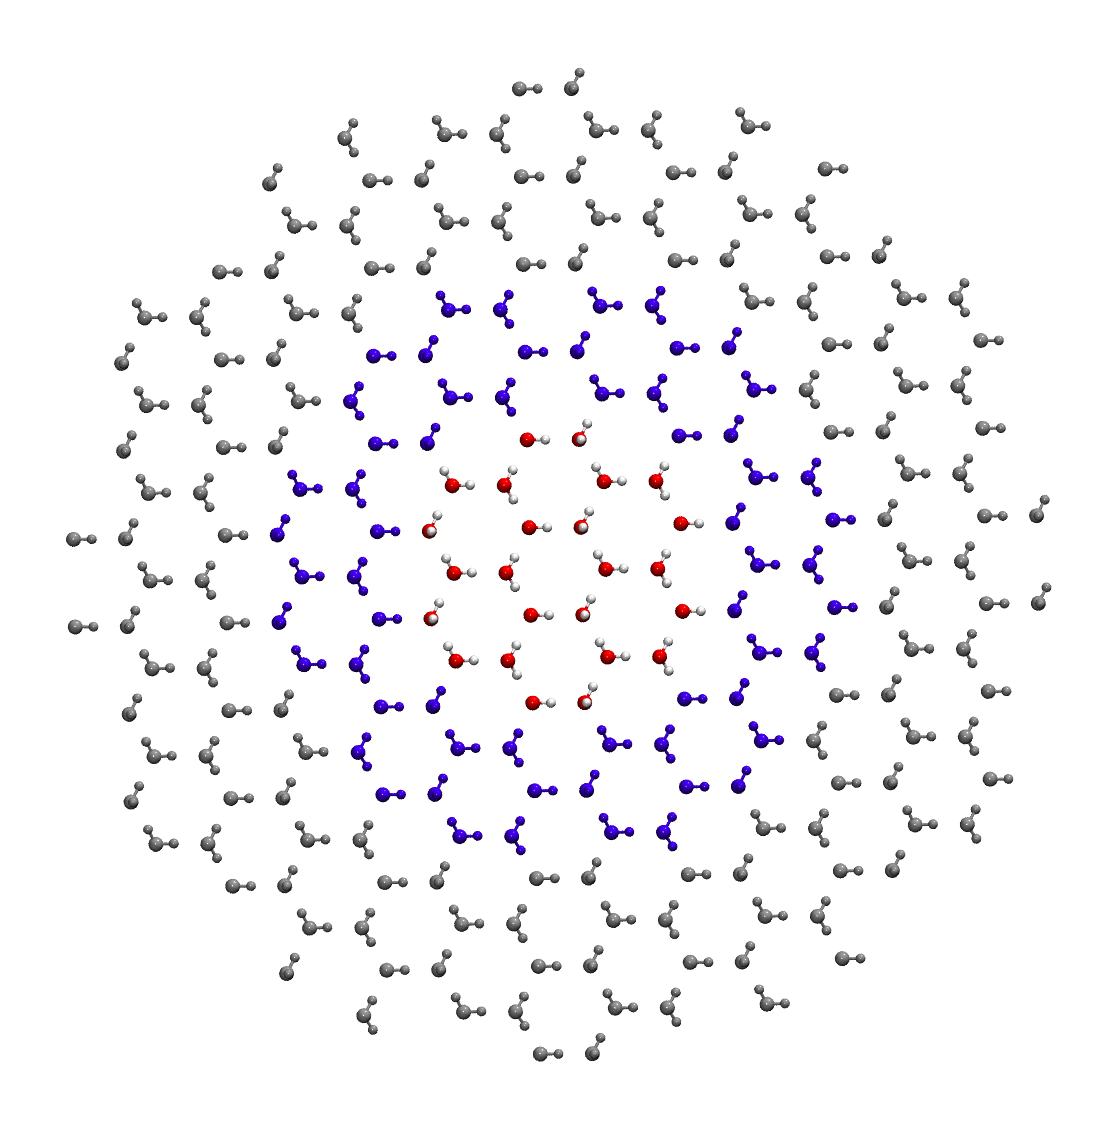
\includegraphics[height=1.8cm]{./TopLayerFromAbove.png}};
%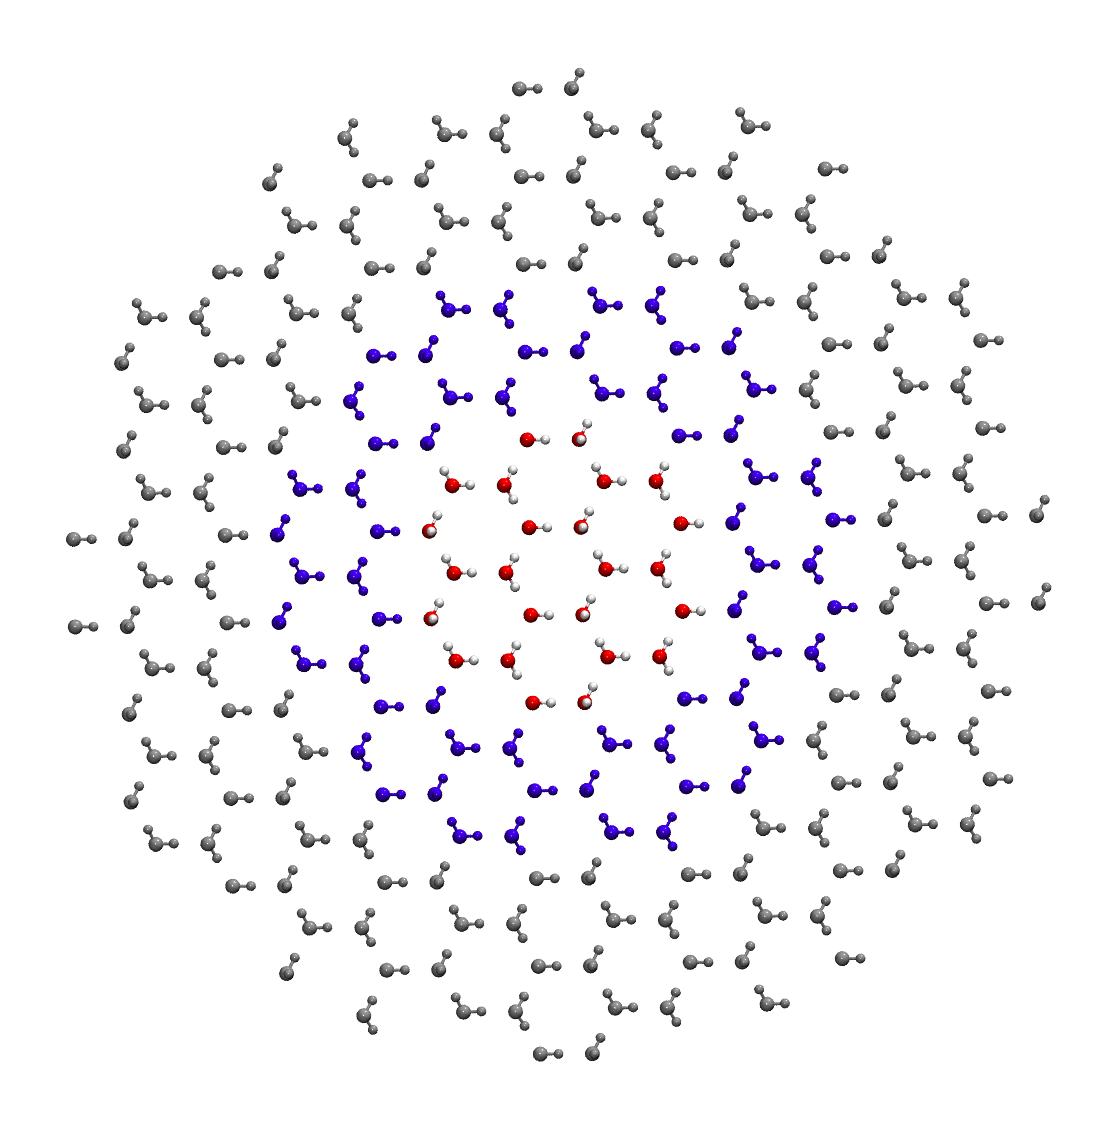
\includegraphics[width=2cm]{./TopLayerFromAbove.png}
%\topsemisphere{gray}{1}
\quicksemisphere{gray}{1.08}{1}

%\draw (2,0) ellipse (1 and 1);

\quicksemisphere{brown}{.61}{.5}
\draw[line width=.2pt,color=gray] (0,0) ellipse (1.08cm and .5*1.08cm);
\shade[ball color=gray!100!white,opacity=.7] (1.08cm,0) arc (0:180:1.08cm and -.5*1.08cm) arc (-180:0:1.08cm and 1.08cm);
%\topsemisphere{gray}{1}
\topsemisphere{blue}{.32}
\shade[ball color=blue!100!white,opacity=.4] (-.32cm,0) arc (-180:-130:.32cm and .32cm) arc (-130:-50:.32cm and .16cm) arc (-50:0:.32cm and .32cm) arc (0:180:.32cm and .16cm);
\draw[color=blue,line width=.2pt] (-.32,0) arc (-180:-130:.32cm and .32cm) arc (-130:-50:.32cm and .16cm) arc (-50:0:.32cm and .32cm) arc (0:180:.32cm and .16cm);
%\quicksemisphere{blue}{.32}{.4}

%\semisphere{red}{220}{.8}{.16}{.08}{.08}

\topsemisphere{red}{.16}
\end{scope}
\end{tikzpicture}
\end{document}